\documentclass[twocolumn]{article}
\usepackage{listings}
\usepackage{amsmath}
\usepackage{fullpage}
\usepackage{tabularx}
\usepackage{graphicx}
\usepackage{caption}
\usepackage{subcaption}
\usepackage{tikz}
\usetikzlibrary{shapes.geometric, arrows}
\usepackage{cite}
\usepackage{hyperref}
\usepackage{float}
\begin{document}
\lstset{language=python, tabsize=4}
\title{Node mapping: a neural network approach to graph mining}
\maketitle

\begin{abstract}
	We present node mapping, a machine learning technique created for numerical 
	link attribute prediction tasks in a graph.
	In this technique, the estimator uses a neural net model to learn to 
	represent every node in the graph as a node vector of real numbers (mapping 
	nodes to vectors), and to learn to predict the target link attribute using 
	these node vectors.
	The main idea is to extract information about nodes from links and to use 
	this information to predict unknown link attributes.
	We demonstrate the usage and high accuracy of this technique in a movie 
	rating prediction task.
\end{abstract}

\section{Introduction}

\subsection{Background}
Both academia and industry have seen pervasive adoption of deep learning 
techniques powered by artificial neural network models since early 2010s,
when they began to outperform other machine learning techniques in various 
application domains (e.g., speech recognition \cite{hannun2014deep}, image 
recognition \cite{simonyan2014very}, and natural language processing 
\cite{yao2013recurrent}).
These neural net models can not only achieve higher prediction accuracy than 
traditional models,
but also require much less domain knowledge and engineering.
Moreover, neural net models have participated in more general artificial 
intelligence design by complementing search techniques, 
demonstrated by Google AlphaGo AI when it defeated go champion Lee Sedol in 
2016 \cite{silver2016mastering}.
Specifically, in a game like go with simple rules but too many possible 
configurations to explore,
neural net models achieve good results with reasonable computing resources, 
which are easily exhausted by algorithms solely powered by search.

\subsection{Motivation}
As neural nets have demonstrated their power in many domains,
we naturally wonder if we can apply them in prediction tasks in graph mining 
domains, 
and what kind of techniques are helpful in using their power.
There are existing techniques with promising results already.
Two earlier attempts were graph neural nets and relational neural 
nets \cite{scarselli2009graph}, 
where neural nets are incorporated into a traditional iterative graph 
information propagation approach.
A later attempt was deep walk \cite{perozzi2014deepwalk}, 
where a graph is reduced to a natural language corpus so that existing neural 
net models designed for natural language processing can handle the graph.
We initiated our research hoping to create a simpler, more direct technique 
that can take advantage of rich information in graphs.
We are particularly interested in application scenarios like making 
recommendations for social network users based on user activities including 
messaging friends, commenting articles, and rating movies.

\subsection{Goal}
We want to create a technique to predict link attributes in a graph using a 
neural net model.
The graph can have any topology and every link can have a numerical attribute.
The estimator should learn to represent the graph in a meaningful way and to 
learn to predict the target link attribute using the representation it learns.

\section{Observations and approach}

\subsection{Entities, representations and relations in different domains}
In order to find out how a neural net can predict link attributes, we first 
review how it handles entities in different domains.
\autoref{tab:domains} provides a summary of various types of entities, their 
numerical representations and inter-entity relations in different domains.
The representations for all the entities are numerical arrays, 
because neural nets rely on neurons' activations and communications, which 
are both numerical.
\begin{table}[h]
	\centering
	\caption{A summary of various types of entities, their numerical
		representations and inter-entity relations in different domains:
		Images and utterances can be directly represented by 2D numerical 
		arrays, 
		but their relations to other images or utterances are not well known. 
		Words in natural languages and nodes in graphs can represented by 
		vectors (1D numerical arrays) and their relations to other words and 
		nodes are well known.}
	\begin{tabularx}{0.5\textwidth}{|X|c|c| }  \hline
 \textbf{Entity} & \textbf{Representation} & \textbf{Relations} \\ \hline
	 image & 2D intensity array & NA \\ \hline
	 utterance & 2D intensity array & NA \\ \hline
	 word & word vector & co-occurrences \\ \hline
	 node & node vector & links \\ \hline
	\end{tabularx}
	\label{tab:domains}
\end{table}

\subsection{Mapping words to vectors}
The famous word2vec technique uses a neural net to learn to map every word in a 
vocabulary to a vector without any domain knowledge \cite{mikolov2013efficient}.
\autoref{tab:word} shows a mapping table that maps each word ID to the word 
vector.
In a corpus, every word is described/defined only by related words in its 
contexts, by implicit relations between words in word co-occurrences.
Nonetheless, the neural net can learn from word co-occurrences and map words to 
vectors accordingly,
such that the relations between words are preserved in the word vector space 
\cite{mikolov2013distributed}.
\begin{table}[h]
	\centering
	\caption{Word to vector mapping table for a vocabulary of size n with word 
		vectors of size d:
		Each word has an ID (words in any language works, e.g., Egyptian).
		The values of vectors in this table are hypothetical.}
	\begin{tabularx}{0.5\textwidth}{|X|X|} \hline
		\textbf{Word ID} & \textbf{Word vector} \\ \hline
		1 & [2.3, 564, -9.5 ... 3] \\ \hline
		2 & [76, -342.2, 0.3 ... 4.2] \\ \hline
		3 & [-345, -834, 0.3 ... 34] \\ \hline
		... & ... \\ \hline
		n & $ [x_1, x_2, x_3 ... x_d] $ \\ \hline
	\end{tabularx}
	\label{tab:word}
\end{table}

\subsection{Mapping nodes to vectors}
\autoref{tab:domains} also shows the similarities between language data and 
graph data.
These similarities suggest a neural net should be able to map nodes to node 
vectors just like mapping words to word vectors.
Moreover, the relations between nodes are explicit (i.e., links),
while relations between words are implicit (i.e., word co-occurrences).
In a social network example, the rating a movie received from a user explicitly 
tells us how much the user likes that movie;
the amount of messages a user sends to another user explicitly tells us how 
much the user likes to talk to the other user.
In a language corpus example, the co-occurrences of words [the, quick, brown, 
fox, jumps, over] implicitly tell us these words are related but do not tell us 
what their relations are.
This observation suggests that a neural net should be able to learn node 
mappings supervised by the link attributes more directly than it learns word 
mappings supervised by word co-occurrences.

\section{Application scenario}

\subsection{Scenario: movie recommendations}
We first demonstrate a simple application scenario on a bipartite graph: 
movie recommendations.
This is a simplified social network where users can only give ratings to movies 
(or like/dislike posts, etc.).
The service provider is interested in recommending movies for each user, solely 
based on the ratings he has given to different movies.

\subsection{Graph: users rating movies}
Formally, the graph is:
\begin{itemize}
	\item a node set consisting of 2 types of nodes: users and movies
	\item a link set consisting of 1 type of links: user-movie links with 
	a numerical attribute - the rating a user has given to a movie
\end{itemize}
If we can build an estimator to predict the rating attributes of unknown 
user-movie links, 
we can know how much a user would like each of the movies he has not 
rated and recommend those he would like the most.

\subsection{Prediction task: movie rating prediction}
Formally, the prediction task is, given any (user, movie) pair, predict the 
rating the user would give to the movie:
\begin{itemize}
	\item input: X = (user, movie)
	\item output: Y = rating(user, movie)
\end{itemize}
This is a common prediction task for recommender systems,
and one of the popular techniques used by these systems is collaborative 
filtering \cite{polatidis2016multi}.
We will compare node mapping against collaborative filtering in this same 
task to see how well our new technique works.

\subsection{Datasets}
There are two recent publications where a large number of collaborative 
filtering variants are benchmarked \cite{hwang2016efficient} 
\cite{polatidis2016multi}. 
\autoref{tab:dataset} shows the specs of 2 datasets used
\cite{harper2015movielens} \footnote{http://grouplens.org/datasets/movielens}.
\autoref{tab:rating} shows a few data samples.
The prediction accuracy metric used is MAE (mean absolute error).
Each dataset is split into 2 parts: 20\% into test set and 80\% 
into training set.
We will conduct the same experiments as in \cite{hwang2016efficient} and  
\cite{polatidis2016multi} and compare the results.
Our estimator sets aside 10\% of the training set as the validation set.
Using larger or smaller validation set doesn't improve the prediction accuracy 
in our experiments.
\begin{table}[h]
	\centering
	\caption{The dataset specs: MovieLens 100K \cite{hwang2016efficient} and 
	MovieLens 1M \cite{polatidis2016multi} datasets.}
	\begin{tabularx}{0.5\textwidth}{ |X|c|c|c|}  \hline
		\textbf{Dataset} & \textbf{users} & \textbf{movies} & \textbf{ratings} 
		\\ \hline
		MovieLens 100K & 1,000 & 1,700 & 100,000 \\ \hline
		MovieLens 1M & 6,000 & 4,000 & 1,000,000 \\ \hline
	\end{tabularx}
	\label{tab:dataset}
\end{table}
\begin{table}[h]
	\centering
	\caption{The dataset samples: Every link has 1 numerical attribute - 
		rating. The rating values in this table are hypothetical.}
	\begin{tabularx}{0.5\textwidth}{ |X|X|X| }  \hline
		\textbf{User ID} & \textbf{Movie ID} & \textbf{Rating} \\ \hline
		0 & 355 & 4 \\ \hline
		0 & 876 & 3 \\ \hline
		0 & 232 & 5 \\ \hline
		... & ... & ... \\ \hline
		999 & 784 & 4 \\ \hline
	\end{tabularx}
	\label{tab:rating}
\end{table}

\section{Solution: neural recommender model}

\subsection{Conceptual model}
Using node mapping technique, we can provide a solution to the recommender 
problem: we create an estimator with a neural net model called neural 
recommender model, shown in \autoref{fig:conceptural}.
\begin{figure*}[h]
	\centering
	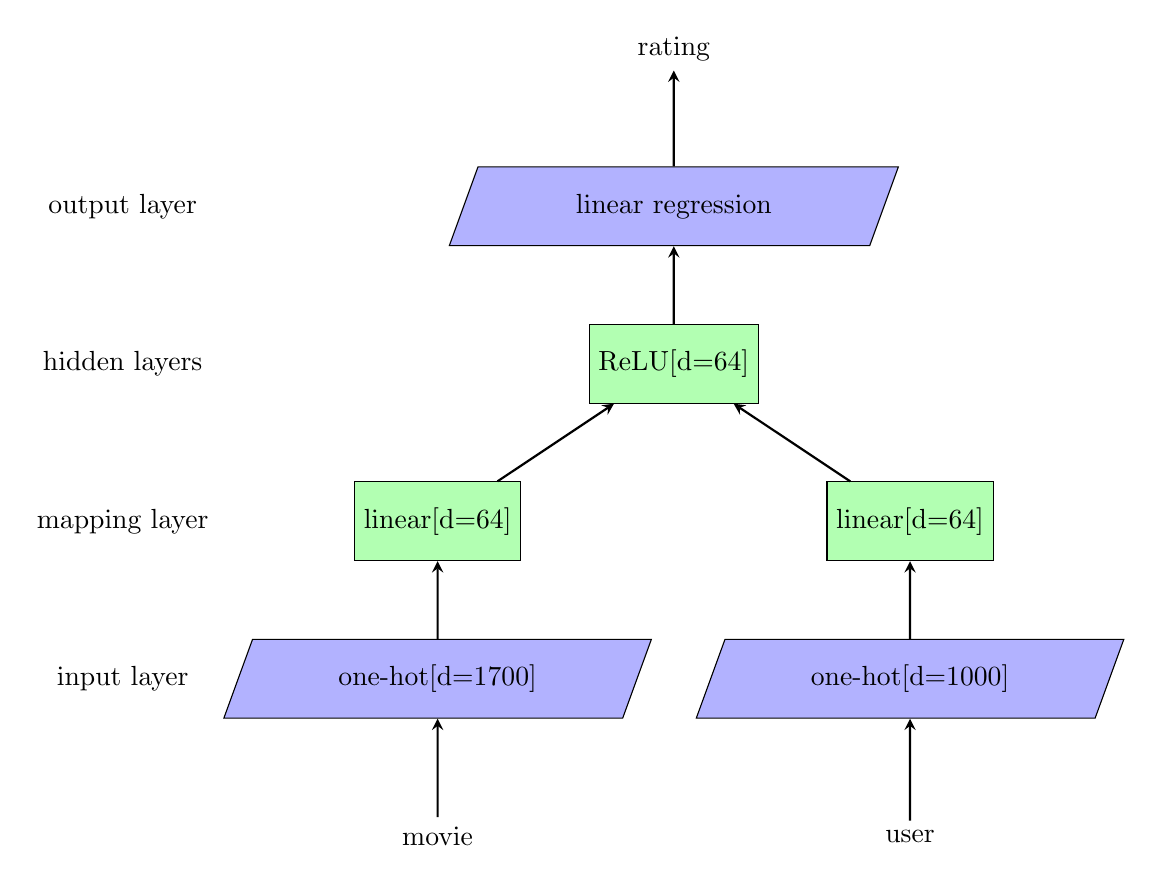
\begin{tikzpicture}[node distance=2cm]
	\tikzstyle{io} = [trapezium, trapezium left angle=70, trapezium right 
	angle=110, minimum width=1cm, minimum height=1cm, text centered, 
	draw=black, fill=blue!30]
	\tikzstyle{process} = [rectangle, minimum width=1cm, minimum height=1cm, 
	text centered, draw=black, fill=green!30]
	\tikzstyle{arrow} = [thick,->,>=stealth]
	\node (linearRegression) [io] {linear regression};
	\node (relu3) [process, below of=linearRegression] {ReLU[d=64]};
	\node (linear2) [process, below of=relu3, xshift=-3cm] {linear[d=64]};
	\node (linear1) [process, below of=relu3, xshift=3cm] {linear[d=64]};
	\node (oneHot2) [io, below of=linear1] {one-hot[d=1000]};
	\node (oneHot1) [io, below of=linear2] {one-hot[d=1700]};
	\node (rating) [above of=linearRegression] {rating};
	\node (output) [left of=linearRegression, xshift=-5cm] {output layer};
	\node (hidden1) [below of=output] {hidden layers};
	\node (mapping) [below of=hidden1] {mapping layer};
	\node (input) [below of=mapping] {input layer};
	\node (movie) [below of=oneHot1] {movie};
	\node (user) [below of=oneHot2] {user};
	\draw [arrow] (movie) -- (oneHot1);
	\draw [arrow] (user) -- (oneHot2);
	\draw [arrow] (oneHot2) -- (linear1);
	\draw [arrow] (oneHot1) -- (linear2);
	\draw [arrow] (linear1) -- (relu3);
	\draw [arrow] (linear2) -- (relu3);
	\draw [arrow] (relu3) -- (linearRegression);
	\draw [arrow] (linearRegression) -- (rating);
	\end{tikzpicture}
	\caption{The conceptual neural recommender model for a dataset with 1700 
	movies and 1000 users:
	The d in the bracket refers to dimension, the layer's size (number of 
	units in the layer).
	We keep all layers the same size for simplicity, although layers of 
	different sizes may produce better results.
	The text before the bracket refers to the activation function of the 
	units in the layer (except for one-hot, which refers to the activations 
	in the input layer).
	Only layers and their connections are shown, while the units in each 
	layer and their connections are not shown.}
	\label{fig:conceptural}
\end{figure*}
The model contains the following layers:
\begin{itemize}
	\item an input layer with one-hot activations: it has 1 channel for movies 
	and 1 channel for users;
	this layer is directly activated by the testing program (e.g., to feed the 
	1200th movie, the testing program sets 1 at the 1200th unit and 0 at other 	
	units in the movie channel);
	\item a mapping layer with linear units: it has 2 channels to map each 
	movie (and each user) to a vector;
	the activations of these 2 channels form the 2 node vectors (i.e., the 
	movie vector and the user vector);
	it is the most critical layer as it gradually learns to map every node to 
	the correct vector during training;
	\item several hidden layers (1 layer is shown in the figure; multiple 
	numbers of layers and layer sizes are experimented) of ReLU 
	(rectified linear unites):
	they have non-linear activation functions to give the model sufficient 
	complexity; 
	they learn to process node vectors and produce more abstract 
	rating-relevant information;
	\item an output layer with a linear regression unit: it learns to predict 
	the rating based on processed information;
\end{itemize}
We fully take into account the characteristics of social networks when 
designing this model.
In a social network, user activities - not user profiles - provide the most 
information about users, so we design the model to learn node vectors 
supervised by link attributes.
We have considered alternative models, but we find them hard to scale.
For example, we can represent a user as the vector of movie ratings he has 
given, 
but this approach will not scale if we have an increasing number of movies.
For example, a new user will require an update to the network topology (at 
least at the input layer) and retraining.

\subsection{Actual model}
In practice, the estimator uses more efficient mapping tables instead of a 
one-hot input layer to handle a graph with increasing number of nodes.
\autoref{fig:actural} shows the actual model with two modifications from the 
conceptual model:
\begin{itemize}
	\item The input layer becomes 2 mapping tables: 1 for movie nodes and 1 
	for user nodes;
	their inputs are node IDs and their outputs are node vectors, just like the 
	word to vector mapping table referenced in \autoref{tab:word}
	\item The mapping layer becomes a 2-channel input layer: it is directly 
	activated by the outputs of the mapping tables
\end{itemize}
\begin{figure*}[h]
	\centering
	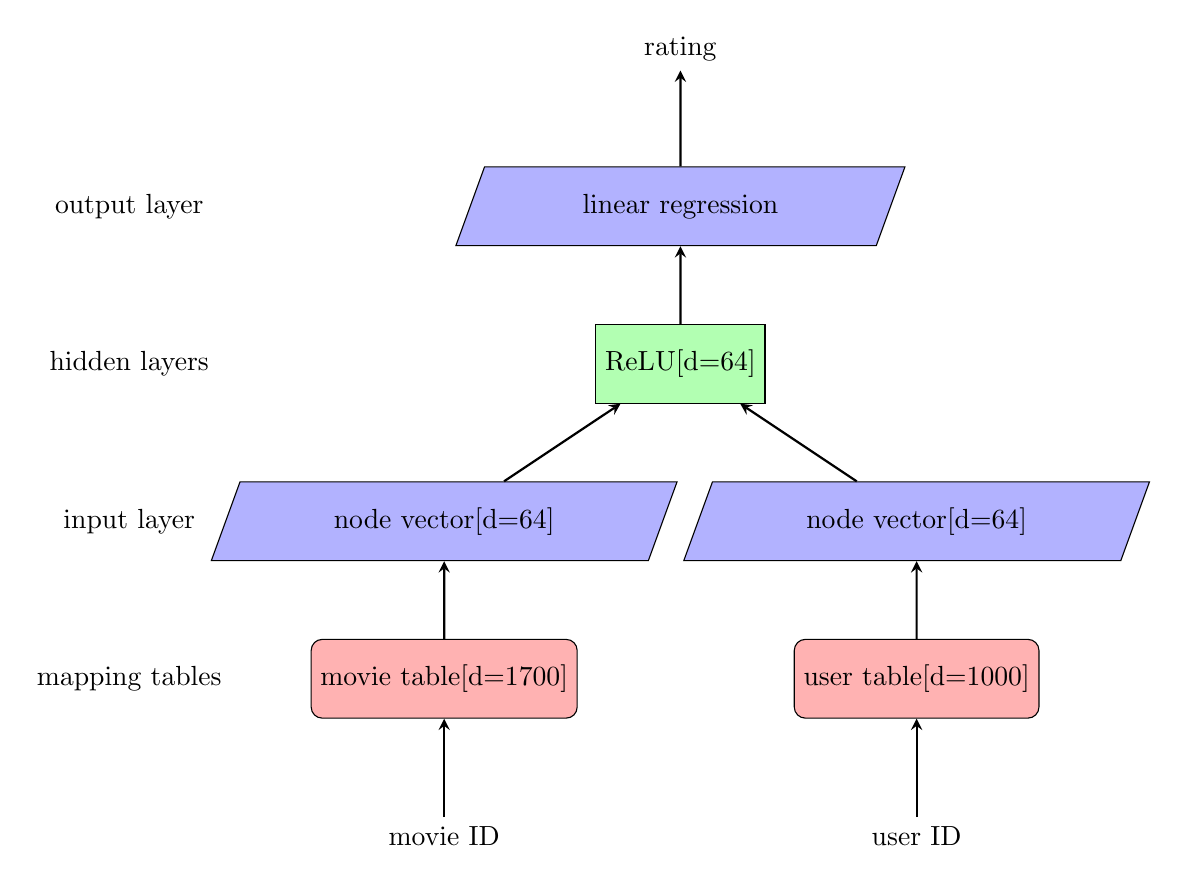
\begin{tikzpicture}[node distance=2cm]
	\tikzstyle{io} = [trapezium, trapezium left angle=70, trapezium right 
	angle=110, minimum width=1cm, minimum height=1cm, text centered, 
	draw=black, fill=blue!30]
	\tikzstyle{startstop} = [rectangle, rounded corners, minimum width=1cm, 
	minimum height=1cm, text centered, draw=black, fill=red!30]
	\tikzstyle{process} = [rectangle, minimum width=1cm, minimum height=1cm, 
	text centered, draw=black, fill=green!30]
	\tikzstyle{arrow} = [thick,->,>=stealth]
	\node (linearRegression) [io] {linear regression};
	\node (relu3) [process, below of=linearRegression] {ReLU[d=64]};
	\node (linear2) [io, below of=relu3, xshift=-3cm] {node vector[d=64]};
	\node (linear1) [io, below of=relu3, xshift=3cm] {node vector[d=64]};
	\node (oneHot2) [startstop, below of=linear1] {user table[d=1000]};
	\node (oneHot1) [startstop, below of=linear2] {movie table[d=1700]};
	\node (rating) [above of=linearRegression] {rating};
	\node (output) [left of=linearRegression, xshift=-5cm] {output layer};
	\node (hidden1) [below of=output] {hidden layers};
	\node (input) [below of=hidden1] {input layer};
	\node (mapping) [below of=input] {mapping tables};
	\node (movie) [below of=oneHot1] {movie ID};
	\node (user) [below of=oneHot2] {user ID};
	\draw [arrow] (movie) -- (oneHot1);
	\draw [arrow] (user) -- (oneHot2);
	\draw [arrow] (oneHot2) -- (linear1);
	\draw [arrow] (oneHot1) -- (linear2);
	\draw [arrow] (linear1) -- (relu3);
	\draw [arrow] (linear2) -- (relu3);
	\draw [arrow] (relu3) -- (linearRegression);
	\draw [arrow] (linearRegression) -- (rating);
	\end{tikzpicture}
	\caption{The actual model with two modifications:
		We factor the node to vector mapping process out of the neural net into 
		2 node to vector mapping tables.
		We feed every node (a movie or user) to the estimator by feeding the 
		node ID.
		During learning, the estimator updates the vectors in the tables the 
		same way it updates weights in the conceptual model.}
	\label{fig:actural}
\end{figure*}

\subsection{Learning techniques}
The estimator uses the above neural net model and a number of popular learning 
techniques:
\begin{itemize}
	\item backpropagation: propagation of the error gradients from output layer 
	back to each earlier layer \cite{rumelhart1988learning}
	\item SGD (stochastic gradient descent): the optimization that minimizes 
	the error (descending against the error gradient in weight space) for a 
	random sample in each step \cite{lecun2012efficient}
	\item mini-batch: the modification to SGD to accelerate and smooth the 
	descent by minimizing the error for a small random portion of samples in 
	each step \cite{mairal2010online}
	\item dropout (specified by keep probability): the technique to reduce unit 
	co-adaptation by temporarily dropping out a random portion of units in each 
	step \cite{srivastava2014dropout}
\end{itemize}

\section{Experiments}

\subsection{Experiment process}
The estimator learns for several epochs.
During each epoch, the estimator updates its model by fitting the training set, 
and then evaluates the learning progress by performing prediction using the 
validation set.
It logs the average training error and average validation error for each epoch 
and stops learning when the validation error starts increasing to reduce 
over-fitting.
This early stopping technique can work well when the validation error 
monotonically decrease to its minimum.
We have not explored more complex early stopping techniques to handle other 
cases.
After learning, the estimator evaluates its model by performing prediction 
using the testing set.
\autoref{fig:trainnig} shows two example learning processes with error traces.
\begin{figure}[h]
	\centering
	\begin{subfigure}{0.4\textwidth}
		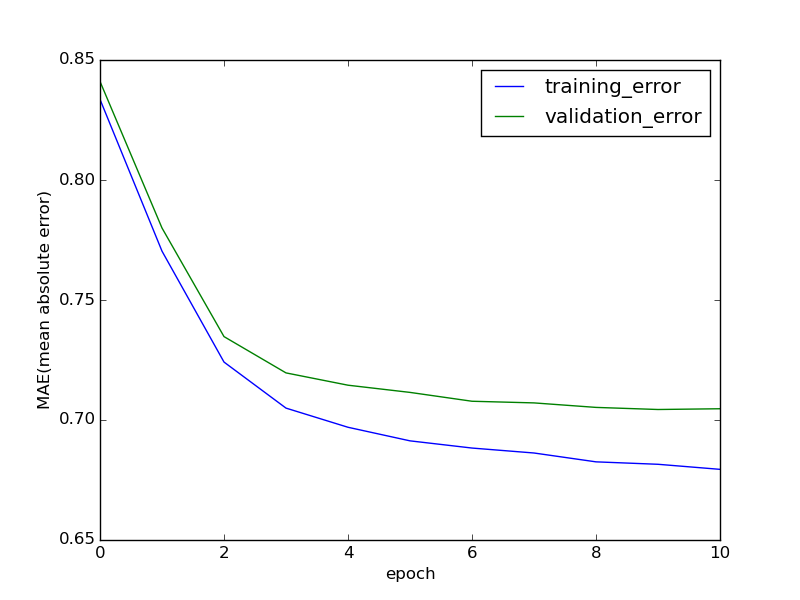
\includegraphics[width=\textwidth]{movieLens100K}
		\caption{MovieLens 100K}
		\label{fig:movieLens100K}
	\end{subfigure}
	\begin{subfigure}{0.4\textwidth}
		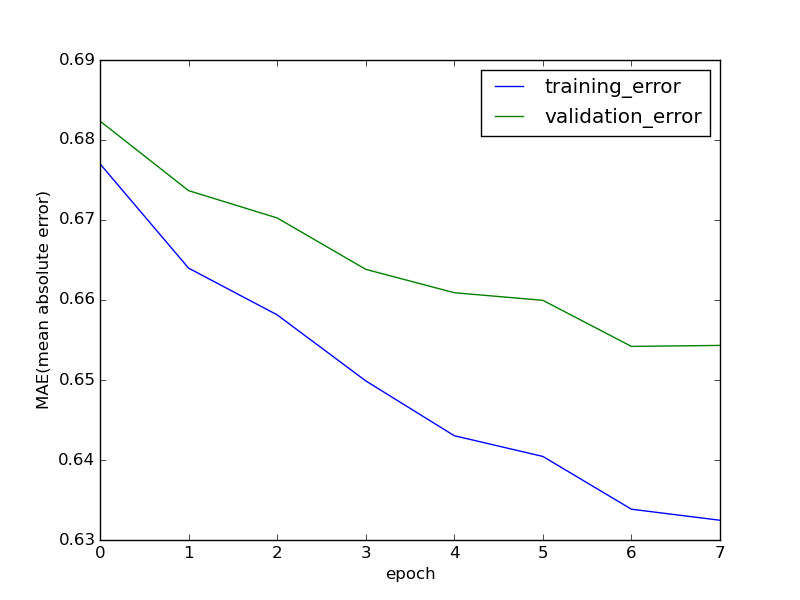
\includegraphics[width=\textwidth]{movieLens1M}
		\caption{MovieLens 1M}
		\label{fig:movieLens1M}
	\end{subfigure}
	\caption{Two example learning processes on different datasets:
	The estimator stops learning when validation errors start increasing at 
	the last epochs. 
	The testing errors are 0.711 for MovieLens 100K and 0.655 for MovieLens 1M.}
	\label{fig:trainnig}
\end{figure}

\subsection{Experiment results: prediction accuracy and estimator robustness}
\autoref{tab:accuracy} shows that neural recommender model outperforms all 
variants of collaborative filtering demonstrated in \cite{hwang2016efficient} 
and \cite{polatidis2016multi}.
\autoref{tab:robust} shows that the estimator is also very robust against 
parameter changes.
\begin{table}[h]
	\centering
	\caption{The comparison of prediction accuracy:
		neural recommender model (NR) has lower errors than collaborative 
		filtering (CF) in both experiments.}
	\begin{tabularx}{0.5\textwidth}{ |X|c|c| }  \hline
		\textbf{Dataset} & \textbf{CF MAE} & \textbf{NR MAE} \\ \hline
		MovieLens 100K & 0.74 & 0.692 \\ \hline
		MovieLens 1M & 0.79 & 0.655 \\ \hline
	\end{tabularx}
	\label{tab:accuracy}
\end{table}
\begin{table*}[h]
	\centering
	\caption{High robustness of the estimator against parameter changes: 
		The estimator maintains testing errors in range [0.69, 0.72] for a wide 
		range of parameters. These experiments are on MovieLens 100K dataset.}
	\begin{tabularx}{\textwidth}{ |X|c|c|c|c| }  \hline
		 \textbf{Learning rate} & \textbf{Keep probability} & \textbf{Layer 
		 size} & \textbf{Number of hidden layers} & \textbf{Testing error} \\ 
		 \hline
		 0.05 & 0.6 & 64 & 2 & 0.7143 \\ \hline
		 0.01 & 0.6 & 64 & 2 & 0.7109 \\ \hline
		 0.1 & 0.6 & 64 & 2 & 0.7114 \\ \hline
		 0.1 & 0.8 & 64 & 2 & 0.7058 \\ \hline
		 0.1 & 0.9 & 64 & 2 & 0.6925 \\ \hline
		 0.1 & 0.9 & 32 & 2 & 0.6965 \\ \hline
		 0.1 & 0.9 & 128 & 2 & 0.7026 \\ \hline
		 0.1 & 0.9 & 32 & 1 & 0.7032 \\ \hline
		 0.1 & 0.9 & 32 & 4 & 0.7008 \\ \hline
	\end{tabularx}
	\label{tab:robust}
\end{table*}

\subsection{Computing resources}
We ran our experiments on a Dell Optiplex 780 with Intel Core 2 Duo CPU and 
each run (learning and prediction) takes around 1 to 8 minutes, 4 to 16 epochs, 
depending on the dataset and parameters.

\section{Strengths}

\subsection{Information mining: node-centered}
This technique takes a node-centered approach as the estimator extracts 
information about nodes from links.
In a social network, this leverages the fact that who a user contacts and what 
movies a user likes tell us what kind of person he is and help us make 
recommendations for him.
It effectively learns complex and unobservable user attributes (node 
attributes) from simple and observable user activities (link attributes). 
\autoref{tab:nodesVSlinks} compares nodes and links with respect to their 
complexity and observability.
\begin{table}[h]
	\centering
	\caption{A comparison of nodes and links with respect to their complexity 
		and attribute observability in a social network:
		Links tend to have low complexity and high observability while nodes 
		are the opposite.
		For example, it is easy to observe simple user activities like sending 
		messages to other users and giving ratings to movies,
		but it is hard to observe complex user attributes like personality, 
		style or taste in movies.}
	\begin{tabularx}{0.5\textwidth}{ |X|c|c| } \hline
		\textbf{Aspect} & \textbf{Node} & \textbf{Link} \\ \hline
		complexity & high & low \\ \hline
		observability & low & high \\ \hline
		example & user & rates, likes, messages \\ \hline
	\end{tabularx}
	\label{tab:nodesVSlinks}
\end{table}

\subsection{Online learning for streaming graphs}
The learning is online when the estimator learns for only one epoch. In 
this case, its prediction accuracy will be lower, but it naturally handles 
streaming graphs:
\begin{itemize}
	\item it can handle a new node by inserting a new vector into the mapping 
	table
	\item it does not need to handle new links as it uses every link once and 
	then discards the link
	\item it does not construct the graph or perform any complex graph 
	operations like neighbor nodes lookup
\end{itemize}
We have not explored more sophisticated techniques for streaming graphs like 
caching a finite set of new links/nodes and learning for multiple epochs on 
that set.

\section{Future work}
In order to generalize this node mapping technique to perform a wider range of 
prediction tasks related to making recommendations for users in a social 
network,
we can consider to work on the following new features for better 
recommendations including friends, groups and posts to users:
\begin{itemize}
	\item handle links connecting two nodes of the same type: e.g., given user 
	A and B, predict the amount of messages A sends to B
	\item handle links with string attributes: e.g., given a text message from 
	user A to user B (a link from A to B with a string attribute), the 
	estimator should learn something about the users from the message content
	\item handle nodes with string attributes: e.g., given an article (a node 
	with a string attribute), the estimator should learn something about the 
	article from the article content
	\item handle links with logical implications: e.g., given a user has 
	written an article (a link from user to article with a write attribute), 
	the estimator should learn something about the user and the article from 
	this activity
\end{itemize}
We have an open source implementation available for interested readers  
\footnote{https://github.com/yuchenhou/elephant}.
The code is in Python and the main machine learning package is TensorFlow 
\cite{abadi2016tensorflow}.
Do not hesitate to contact us if you are interested in collaboration.

\section{Conclusions}
Node mapping is an effective technique to predict link attributes in a graph 
using a neural net model.
The estimator learns both to represent each node with a vector, and to predict 
the target link attribute using these vectors.
It achieves better rating prediction accuracy than collaborative filtering and 
many of its variants.
For recommendation tasks in social networks, this technique coincides with the 
idea of understanding complex users from their simple activities, and using 
that understanding to predict their future activities.

\bibliographystyle{plain}
\bibliography{references}

\end{document}
